\begin{figure}[H]
\centering
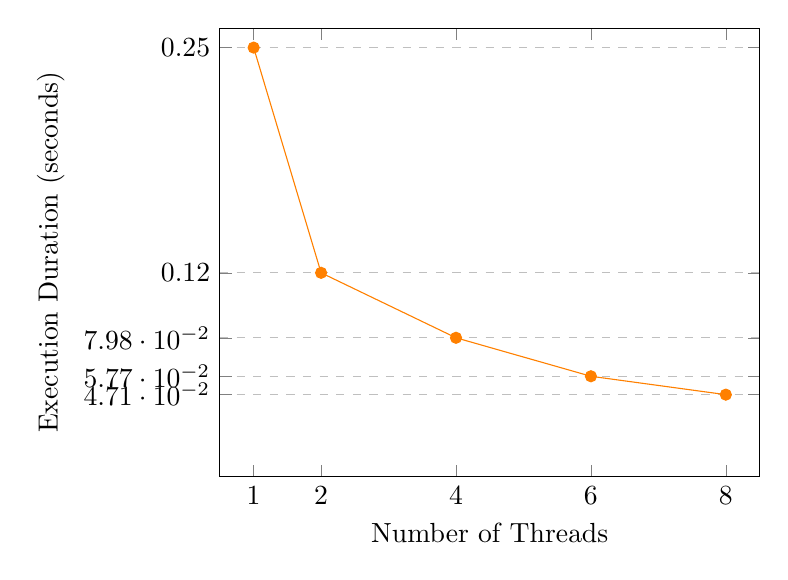
\begin{tikzpicture}
\begin{axis}[
    xlabel={Number of Threads},
    ylabel={Execution Duration (seconds)},
    xmin=0.5, xmax=8.5,
    ymin=0, ymax=0.258,
    xtick={1, 2, 4, 6, 8},
    ytick={.246844327, .117240608, .079848087, .057706782, .047123577},
    ymajorgrids=true,
    grid style=dashed,
]

\addplot[
    color=orange,
    mark=*,
    ]
    coordinates {
    (1,.246844327) (2,.117240608) (4,.079848087) (6,.057706782) (8,.047123577)
    };

\end{axis}
\end{tikzpicture}
\caption{Execution Duration vs. Number of Threads for Isolation}
\label{fig:isolation}
\end{figure}